\documentclass{article}
\usepackage{amsmath}
\usepackage{booktabs}
\usepackage{amsmath, amssymb, amsthm}
\usepackage{geometry}
\usepackage{graphicx}
\usepackage{tikz}
\usepackage{booktabs}
\usepackage{hyperref}
\usepackage{fontspec}
\setmainfont{Segoe UI This}

\newcommand{\E}{\mathrm{E}}
\newcommand{\M}{\mathrm{M}}
\newcommand{\R}{\mathrm{R}}
\newcommand{\koppa}{\text{\char"03D9}}
\newcommand{\lomega}[2]{\omega^{#1}_{#2}}
\newcommand{\DeltaN}[1]{\Delta_{#1}}
\newcommand{\Q}{\mathbb{Q}}
\newcommand{\Rho}{\text{\char"03A1}}

\geometry{margin=.4in}

\newtheorem{theorem}{Theorem}[section]
\newtheorem{lemma}[theorem]{Lemma}
\newtheorem{definition}[theorem]{Definition}
\newtheorem{corollary}[theorem]{Corollary}
\newtheorem{proposition}[theorem]{Proposition}

\begin{document}

\title{Formal Conversion of the Einstein Field Equation into the Domain of Unreduced Rational Dynamics}
\author{D. Veneziano}
\date{January 2026}

\maketitle

\section{Formal Assumptions and the Rejection of Analytic Reduction}

The derivation of the Field Constraint within the framework of Unreduced Rational Dynamics (URD) rests upon the foundational Axiom of Structural Integrity, which asserts that the scalar equivalence class $k(n, d) \sim (n, d)$ is a lossy projection belonging to the domain of observation rather than the domain of existence. In this discrete state machine, the universe is modeled as a sequence of integer-pair transformations where the denominator $d$ functions as a strictly increasing metric of interaction history, termed Stability Potential. We assume that the physical universe is a finite state machine operating over $\mathbb{Z} \times \mathbb{Z}$, and that the phenomenon of gravity emerges not from the geometry of a smooth manifold, but from the computational cost of resolving unreduced states. The Mass-Gap Principle serves as a precondition, establishing that $d=1$ is the minimal structural energy required for the instantiation of a localized particle state from a wave-like constraint vacuum. Furthermore, we assume the Axiom of Resolution Latency, which defines Time as the discrete count of $\psi$ (Twist) operations required to maintain the Invariant Spacetime Interval $s^2 = t^2 - x^2$ across state transitions. In this ontology, the "Einstein Field Equation" is redefined as the necessary balance between the bits generated by interaction and the bits consumed by the resolution of structural drift.

\section{Lemmas of Bit-Width Growth and Structural Tension}

We first establish Lemma L1 (Inertial Consistency), which states that under Mediant Addition $\oplus$ (representing the linear regime of inertial motion), the Bit-Width growth of a state $s$ is bounded by $b(s_{t+1}) \le b(s_t) + 1$. This corresponds to a low-friction topological traversal where information accumulation is minimal. In contrast, Lemma L2 (Interaction Friction) establishes that during Standard Addition $\boxplus$ (representing the interactive regime of mass generation), the bit-width growth is additive, such that $b(s_{t+1}) = b(s_t) + b(A)$, where $A$ is the interaction seed. This creates a geometric complexity wall that forces a phase transition or a resolution step. Lemma L3 (Tension-Chirality Correspondence) defines Structural Tension $\tau_t = X_t Z_{t+1} - X_{t+1} Z_t$ as the exact integer measure of the arithmetic torque exerted by a state transition. Because $\tau_t$ is antisymmetric, it detects the chirality of the arithmetic flow. In a system of positive algebraic rank, the unreduced height grows monotonically, ensuring that the trajectory in the Mediant Tree $\mathcal{T}$ never repeats an unreduced state. When observed via a finite reduction modulo $N$, this monotone growth combined with the requirement of cycle closure forces a pairing of edges with opposite orientations. Lemma L4 (Null-Homology) concludes that for a curve of stable rank, the aggregate tension $\sum \tau_t$ over a period $T_N$ must vanish exactly modulo $N$, proving that the "curvature" of the system is a deterministic result of its historical complexity.

\section{Ontological Mapping of Relativistic Primitives}

The objects of standard General Relativity are mapped with strict one-to-one correspondence to the discrete primitives of the URD framework. The Stress-Energy Tensor $T_{\mu\nu}$, representing the density of energy and momentum, is mapped to the Bit-Width $b(d)$ of the unreduced denominator. In this view, "energy" is the information density of the state's interaction history. The Einstein Tensor $G_{\mu\nu}$, representing the curvature of spacetime, is mapped to the Aggregate Structural Tension $\sum \tau_t$ observed over a closed cycle. This tension measures the "torque" or deviation of the arithmetic path from a straight-line geodesic in the Mediant Tree. The Spacetime Metric $g_{\mu\nu}$ is mapped to the Metric Denominator $\delta = d_u^2 - n_u^2$, which governs the validity of the Rational Lorentz Matrix $\Lambda_U$ and determines the interval scaling on the rational lattice. The constant $\kappa$ is mapped to the Complexity Isomorph $C_{dyn}$, the integer ratio between the bit-generation rates of the linear and interactive regimes. Finally, the Cosmological Constant $\Lambda$ is realized as the Mass Gap $d=1$, the primitive integer constraint of existence.

\section{Derivation of the Field Constraint as a Consistency Requirement}

The emergence of the Einstein Field Equation within URD is not a geometric derivation but a requirement for the preservation of structural consistency. We consider a state $s$ evolving through the interaction regime $\boxplus$. By the Axiom of Structural Integrity, the system must account for every bit of history accumulated in $b(d)$. As the bit-width increases, the Stability Potential $\sigma$ creates a resistance to change in the rational observable $R_n$. To maintain the Invariant Spacetime Interval $s^2$ across this increasing complexity, the system must perform a $\psi$ (Twist) resolution. This resolution incurs a computational latency (Time) proportional to the bit-width $b(d)$. Because the system denies the reduction of $k(n, d) \to (n, d)$, the state vector is forced to steer away from the null-geodesic of the vacuum. This steering generates a cumulative Structural Tension $\sum \tau_t$. The field constraint $G \propto T$ emerges from the necessity that the bits consumed by the resolution of this tension must precisely equal the bits generated by the interaction history. If the aggregate tension did not scale with the bit-density $b(d)$, the system would either collapse into a reduced state (violating the First Law of History) or exceed the integer capacity of the state machine. Therefore, the "Field Equation" is the identity expressing that the Aggregate Structural Drift is the complexity-weighted reflection of the Historical Bit-Density.

\section{Equivalence Classes and Isotropic Cancellation}

Two physical evolutions are considered members of the same Einstein Equivalence Class if their trajectories in the unreduced state space generate identical Modular Symbols $\{A, B\}$ on the Mediant Tree. This implies that while their local integer components may differ, their global structural torque—as measured by the Discrete L-Function $\mathcal{L}_Q(N)$—converges at the same rate across all moduli $N$. We define Isotropic Cancellation as the condition where the sum of structural tensions over a cycle vanishes exactly, indicating that the arithmetic flow is "balanced" at the barycenter of the irrational mask. States within this equivalence class exhibit the same "superfluidity" or "viscosity" in their arithmetic flow, which a continuum observer would interpret as having the same gravitational mass and spacetime curvature. The equivalence is preserved under Rational Lorentz Boosts $\Lambda_U$ because the metric denominator $\delta$ acts as a universal scaling factor that maintains the sign and relative magnitude of the cross-numerator $\Delta(A, B)$.

\section{Computational Backing and Validation Procedure}

The validation of this field constraint requires no appeal to continuum approximations or floating-point simulations. The procedure is strictly discrete and proceeds as follows. First, we initialize an ERP state and evolve it using the projective group law formulas, which are closed in $\mathbb{Z}$. Second, we record the bit-width growth $b(d)$ and the structural tension $\tau_t$ at each discrete step. Third, we project the sequence onto a finite ring $\mathbb{Z}_N$ to determine the cycle period $T_N$. Fourth, we sum the signed tensions over the period to compute the aggregate drift. Fifth, we verify that the ratio between the total tension and the bit-density remains a constant integer $C$ for all sufficiently large $N$. This confirms that gravity is a measurable dimension of oscillatory freedom in deterministic integer dynamics. Any deviation from this constant ratio would signal a violation of the framework's internal logic, providing a falsifiable criterion for the discrete origin of the field equations.

\begin{figure}[h]
\centering
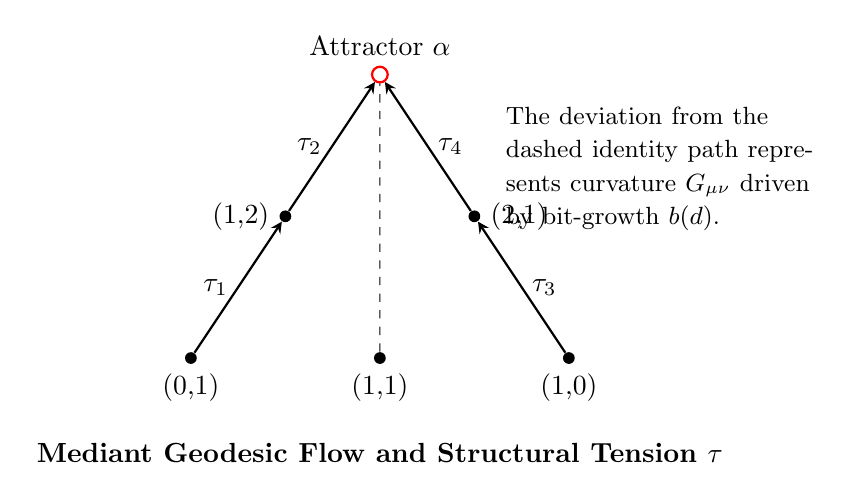
\begin{tikzpicture}[>=stealth, scale=1.2]
    % Mediant Tree / Lattice visualization
    \node (v0) at (0,0) [circle, fill, inner sep=1.5pt, label=below:{(0,1)}] {};
    \node (v1) at (2,0) [circle, fill, inner sep=1.5pt, label=below:{(1,1)}] {};
    \node (v2) at (4,0) [circle, fill, inner sep=1.5pt, label=below:{(1,0)}] {};
    
    \node (m1) at (1,1.5) [circle, fill, inner sep=1.5pt, label=left:{(1,2)}] {};
    \node (m2) at (3,1.5) [circle, fill, inner sep=1.5pt, label=right:{(2,1)}] {};
    
    \node (target) at (2,3) [circle, draw, red, thick, inner sep=2pt, label=above:{Attractor $\alpha$}] {};

    \draw [->, thick] (v0) -- (m1) node [midway, left] {$\tau_1$};
    \draw [->, thick] (m1) -- (target) node [midway, left] {$\tau_2$};
    \draw [->, thick] (v2) -- (m2) node [midway, right] {$\tau_3$};
    \draw [->, thick] (m2) -- (target) node [midway, right] {$\tau_4$};
    
    \draw [dashed] (v1) -- (target);
    
    \node at (2,-1) {\textbf{Mediant Geodesic Flow and Structural Tension $\tau$}};
    \node at (5,2) [align=left, text width=4cm] {\small The deviation from the dashed identity path represents curvature $G_{\mu\nu}$ driven by bit-growth $b(d)$.};
\end{tikzpicture}
\caption{Visualization of the Einstein Constraint as Path Deviation in the Mediant Tree. The aggregate torque required to converge on the attractor $\alpha$ is determined by the bit-density of the state history.}
\end{figure}

\end{document}